\documentclass[twoside]{book}

% Packages required by doxygen
\usepackage{fixltx2e}
\usepackage{calc}
\usepackage{doxygen}
\usepackage{graphicx}
\usepackage[utf8]{inputenc}
\usepackage{makeidx}
\usepackage{multicol}
\usepackage{multirow}
\PassOptionsToPackage{warn}{textcomp}
\usepackage{textcomp}
\usepackage[nointegrals]{wasysym}
\usepackage[table]{xcolor}

% Font selection
\usepackage[T1]{fontenc}
\usepackage{mathptmx}
\usepackage[scaled=.90]{helvet}
\usepackage{courier}
\usepackage{amssymb}
\usepackage{sectsty}
\renewcommand{\familydefault}{\sfdefault}
\allsectionsfont{%
  \fontseries{bc}\selectfont%
  \color{darkgray}%
}
\renewcommand{\DoxyLabelFont}{%
  \fontseries{bc}\selectfont%
  \color{darkgray}%
}
\newcommand{\+}{\discretionary{\mbox{\scriptsize$\hookleftarrow$}}{}{}}

% Page & text layout
\usepackage{geometry}
\geometry{%
  a4paper,%
  top=2.5cm,%
  bottom=2.5cm,%
  left=2.5cm,%
  right=2.5cm%
}
\tolerance=750
\hfuzz=15pt
\hbadness=750
\setlength{\emergencystretch}{15pt}
\setlength{\parindent}{0cm}
\setlength{\parskip}{0.2cm}
\makeatletter
\renewcommand{\paragraph}{%
  \@startsection{paragraph}{4}{0ex}{-1.0ex}{1.0ex}{%
    \normalfont\normalsize\bfseries\SS@parafont%
  }%
}
\renewcommand{\subparagraph}{%
  \@startsection{subparagraph}{5}{0ex}{-1.0ex}{1.0ex}{%
    \normalfont\normalsize\bfseries\SS@subparafont%
  }%
}
\makeatother

% Headers & footers
\usepackage{fancyhdr}
\pagestyle{fancyplain}
\fancyhead[LE]{\fancyplain{}{\bfseries\thepage}}
\fancyhead[CE]{\fancyplain{}{}}
\fancyhead[RE]{\fancyplain{}{\bfseries\leftmark}}
\fancyhead[LO]{\fancyplain{}{\bfseries\rightmark}}
\fancyhead[CO]{\fancyplain{}{}}
\fancyhead[RO]{\fancyplain{}{\bfseries\thepage}}
\fancyfoot[LE]{\fancyplain{}{}}
\fancyfoot[CE]{\fancyplain{}{}}
\fancyfoot[RE]{\fancyplain{}{\bfseries\scriptsize Generated on Sun Sep 28 2014 02\+:39\+:45 for Simphplist by Doxygen }}
\fancyfoot[LO]{\fancyplain{}{\bfseries\scriptsize Generated on Sun Sep 28 2014 02\+:39\+:45 for Simphplist by Doxygen }}
\fancyfoot[CO]{\fancyplain{}{}}
\fancyfoot[RO]{\fancyplain{}{}}
\renewcommand{\footrulewidth}{0.4pt}
\renewcommand{\chaptermark}[1]{%
  \markboth{#1}{}%
}
\renewcommand{\sectionmark}[1]{%
  \markright{\thesection\ #1}%
}

% Indices & bibliography
\usepackage{natbib}
\usepackage[titles]{tocloft}
\setcounter{tocdepth}{3}
\setcounter{secnumdepth}{5}
\makeindex

% Hyperlinks (required, but should be loaded last)
\usepackage{ifpdf}
\ifpdf
  \usepackage[pdftex,pagebackref=true]{hyperref}
\else
  \usepackage[ps2pdf,pagebackref=true]{hyperref}
\fi
\hypersetup{%
  colorlinks=true,%
  linkcolor=blue,%
  citecolor=blue,%
  unicode%
}

% Custom commands
\newcommand{\clearemptydoublepage}{%
  \newpage{\pagestyle{empty}\cleardoublepage}%
}


%===== C O N T E N T S =====

\begin{document}

% Titlepage & ToC
\hypersetup{pageanchor=false,
             bookmarks=true,
             bookmarksnumbered=true,
             pdfencoding=unicode
            }
\pagenumbering{roman}
\begin{titlepage}
\vspace*{7cm}
\begin{center}%
{\Large Simphplist \\[1ex]\large 0.\+1.\+0 }\\
\vspace*{1cm}
{\large Generated by Doxygen 1.8.8}\\
\vspace*{0.5cm}
{\small Sun Sep 28 2014 02:39:45}\\
\end{center}
\end{titlepage}
\clearemptydoublepage
\tableofcontents
\clearemptydoublepage
\pagenumbering{arabic}
\hypersetup{pageanchor=true}

%--- Begin generated contents ---
\chapter{Overview}
\label{index}\hypertarget{index}{}Simphplist is a mini-\/framework with anti-\/framework features. A collection of losely coupled components, that helps you with shortcuts and clean A\+P\+I's for writing the most common idioms when developing web applications in P\+H\+P (My\+S\+Q\+L handling, object mapper, authentication, validation, typechecking).

You can use it as a minimalistic base for writing custom (frameworks for) applications. Simphplist is carefully designed to allow using it alongside any other (custom) framework.\hypertarget{index_license}{}\section{License}\label{index_license}
Copyright (c) 2014 Benjamin Althues \href{mailto:benjamin@babab.nl}{\tt benjamin@babab.\+nl}

Permission to use, copy, modify, and distribute this software for any purpose with or without fee is hereby granted, provided that the above copyright notice and this permission notice appear in all copies.

T\+H\+E S\+O\+F\+T\+W\+A\+R\+E I\+S P\+R\+O\+V\+I\+D\+E\+D \char`\"{}\+A\+S I\+S\char`\"{} A\+N\+D T\+H\+E A\+U\+T\+H\+O\+R D\+I\+S\+C\+L\+A\+I\+M\+S A\+L\+L W\+A\+R\+R\+A\+N\+T\+I\+E\+S W\+I\+T\+H R\+E\+G\+A\+R\+D T\+O T\+H\+I\+S S\+O\+F\+T\+W\+A\+R\+E I\+N\+C\+L\+U\+D\+I\+N\+G A\+L\+L I\+M\+P\+L\+I\+E\+D W\+A\+R\+R\+A\+N\+T\+I\+E\+S O\+F M\+E\+R\+C\+H\+A\+N\+T\+A\+B\+I\+L\+I\+T\+Y A\+N\+D F\+I\+T\+N\+E\+S\+S. I\+N N\+O E\+V\+E\+N\+T S\+H\+A\+L\+L T\+H\+E A\+U\+T\+H\+O\+R B\+E L\+I\+A\+B\+L\+E F\+O\+R A\+N\+Y S\+P\+E\+C\+I\+A\+L, D\+I\+R\+E\+C\+T, I\+N\+D\+I\+R\+E\+C\+T, O\+R C\+O\+N\+S\+E\+Q\+U\+E\+N\+T\+I\+A\+L D\+A\+M\+A\+G\+E\+S O\+R A\+N\+Y D\+A\+M\+A\+G\+E\+S W\+H\+A\+T\+S\+O\+E\+V\+E\+R R\+E\+S\+U\+L\+T\+I\+N\+G F\+R\+O\+M L\+O\+S\+S O\+F U\+S\+E, D\+A\+T\+A O\+R P\+R\+O\+F\+I\+T\+S, W\+H\+E\+T\+H\+E\+R I\+N A\+N A\+C\+T\+I\+O\+N O\+F C\+O\+N\+T\+R\+A\+C\+T, N\+E\+G\+L\+I\+G\+E\+N\+C\+E O\+R O\+T\+H\+E\+R T\+O\+R\+T\+I\+O\+U\+S A\+C\+T\+I\+O\+N, A\+R\+I\+S\+I\+N\+G O\+U\+T O\+F O\+R I\+N C\+O\+N\+N\+E\+C\+T\+I\+O\+N W\+I\+T\+H T\+H\+E U\+S\+E O\+R P\+E\+R\+F\+O\+R\+M\+A\+N\+C\+E O\+F T\+H\+I\+S S\+O\+F\+T\+W\+A\+R\+E. 
\chapter{Namespace Index}
\section{Namespace List}
Here is a list of all documented namespaces with brief descriptions\+:\begin{DoxyCompactList}
\item\contentsline{section}{\hyperlink{namespaceBabab}{Babab} \\*Vendor namespace of developer Benjamin Althues (babab.\+nl) }{\pageref{namespaceBabab}}{}
\item\contentsline{section}{\hyperlink{namespaceBabab_1_1Simphplist}{Babab\+::\+Simphplist} \\*Framework namespace }{\pageref{namespaceBabab_1_1Simphplist}}{}
\item\contentsline{section}{\hyperlink{namespaceBabab_1_1Simphplist_1_1Auth}{Babab\+::\+Simphplist\+::\+Auth} \\*Authentication of Users Library }{\pageref{namespaceBabab_1_1Simphplist_1_1Auth}}{}
\item\contentsline{section}{\hyperlink{namespaceBabab_1_1Simphplist_1_1DB}{Babab\+::\+Simphplist\+::\+D\+B} \\*My\+S\+Q\+L Handling and simplistic Object Mapper with a clean A\+P\+I }{\pageref{namespaceBabab_1_1Simphplist_1_1DB}}{}
\item\contentsline{section}{\hyperlink{namespaceBabab_1_1SimphplistTests}{Babab\+::\+Simphplist\+Tests} \\*Unit tests namespace }{\pageref{namespaceBabab_1_1SimphplistTests}}{}
\end{DoxyCompactList}

\chapter{Hierarchical Index}
\section{Class Hierarchy}
This inheritance list is sorted roughly, but not completely, alphabetically\+:\begin{DoxyCompactList}
\item \contentsline{section}{Babab\textbackslash{}Simphplist\textbackslash{}Auth\textbackslash{}Cookie\+Auth}{\pageref{classBabab_1_1Simphplist_1_1Auth_1_1CookieAuth}}{}
\item \contentsline{section}{Babab\textbackslash{}Simphplist\textbackslash{}Debug}{\pageref{classBabab_1_1Simphplist_1_1Debug}}{}
\item \contentsline{section}{Babab\textbackslash{}Simphplist\textbackslash{}Json}{\pageref{classBabab_1_1Simphplist_1_1Json}}{}
\item \contentsline{section}{Babab\textbackslash{}Simphplist\textbackslash{}D\+B\textbackslash{}Model\+Interface}{\pageref{interfaceBabab_1_1Simphplist_1_1DB_1_1ModelInterface}}{}
\begin{DoxyCompactList}
\item \contentsline{section}{Babab\textbackslash{}Simphplist\textbackslash{}D\+B\textbackslash{}Model}{\pageref{classBabab_1_1Simphplist_1_1DB_1_1Model}}{}
\begin{DoxyCompactList}
\item \contentsline{section}{Babab\textbackslash{}Simphplist\textbackslash{}D\+B\textbackslash{}Model\+Test}{\pageref{classBabab_1_1Simphplist_1_1DB_1_1ModelTest}}{}
\end{DoxyCompactList}
\end{DoxyCompactList}
\item \contentsline{section}{Babab\textbackslash{}Simphplist\textbackslash{}D\+B\textbackslash{}Mysql\+Handler}{\pageref{classBabab_1_1Simphplist_1_1DB_1_1MysqlHandler}}{}
\item P\+H\+P\+Unit\+\_\+\+Framework\+\_\+\+Test\+Case\begin{DoxyCompactList}
\item \contentsline{section}{Babab\textbackslash{}Simphplist\+Tests\textbackslash{}String\+Test}{\pageref{classBabab_1_1SimphplistTests_1_1StringTest}}{}
\end{DoxyCompactList}
\item \contentsline{section}{Babab\textbackslash{}Simphplist\textbackslash{}Request}{\pageref{classBabab_1_1Simphplist_1_1Request}}{}
\item \contentsline{section}{Babab\textbackslash{}Simphplist\textbackslash{}Route}{\pageref{classBabab_1_1Simphplist_1_1Route}}{}
\item \contentsline{section}{Babab\textbackslash{}Simphplist\textbackslash{}String}{\pageref{classBabab_1_1Simphplist_1_1String}}{}
\item \contentsline{section}{Babab\textbackslash{}Simphplist\textbackslash{}Validate}{\pageref{classBabab_1_1Simphplist_1_1Validate}}{}
\end{DoxyCompactList}

\chapter{Class Index}
\section{Class List}
Here are the classes, structs, unions and interfaces with brief descriptions\+:\begin{DoxyCompactList}
\item\contentsline{section}{\hyperlink{classBabab_1_1Simphplist_1_1Auth_1_1CookieAuth}{Babab\textbackslash{}\+Simphplist\textbackslash{}\+Auth\textbackslash{}\+Cookie\+Auth} \\*Authenticate a user with a persistent login token cookie }{\pageref{classBabab_1_1Simphplist_1_1Auth_1_1CookieAuth}}{}
\item\contentsline{section}{\hyperlink{classBabab_1_1Simphplist_1_1Debug}{Babab\textbackslash{}\+Simphplist\textbackslash{}\+Debug} \\*Static methods for dumping vars to a file or screen (html or text) }{\pageref{classBabab_1_1Simphplist_1_1Debug}}{}
\item\contentsline{section}{\hyperlink{classBabab_1_1Simphplist_1_1Json}{Babab\textbackslash{}\+Simphplist\textbackslash{}\+Json} \\*Shortcuts for common idioms in J\+S\+O\+N interaction }{\pageref{classBabab_1_1Simphplist_1_1Json}}{}
\item\contentsline{section}{\hyperlink{classBabab_1_1Simphplist_1_1DB_1_1Model}{Babab\textbackslash{}\+Simphplist\textbackslash{}\+D\+B\textbackslash{}\+Model} \\*Object Mapper -- Abstract base class for writing Models that will be mapped to database tables }{\pageref{classBabab_1_1Simphplist_1_1DB_1_1Model}}{}
\item\contentsline{section}{\hyperlink{interfaceBabab_1_1Simphplist_1_1DB_1_1ModelInterface}{Babab\textbackslash{}\+Simphplist\textbackslash{}\+D\+B\textbackslash{}\+Model\+Interface} \\*P\+H\+P Interface for abstract base class \hyperlink{classBabab_1_1Simphplist_1_1DB_1_1Model}{Model} }{\pageref{interfaceBabab_1_1Simphplist_1_1DB_1_1ModelInterface}}{}
\item\contentsline{section}{\hyperlink{classBabab_1_1Simphplist_1_1DB_1_1ModelTest}{Babab\textbackslash{}\+Simphplist\textbackslash{}\+D\+B\textbackslash{}\+Model\+Test} \\*Test model used as code example / for unit testing }{\pageref{classBabab_1_1Simphplist_1_1DB_1_1ModelTest}}{}
\item\contentsline{section}{\hyperlink{classBabab_1_1Simphplist_1_1DB_1_1MysqlHandler}{Babab\textbackslash{}\+Simphplist\textbackslash{}\+D\+B\textbackslash{}\+Mysql\+Handler} \\*My\+S\+Q\+L Handler with table prefix support }{\pageref{classBabab_1_1Simphplist_1_1DB_1_1MysqlHandler}}{}
\item\contentsline{section}{\hyperlink{classBabab_1_1Simphplist_1_1Request}{Babab\textbackslash{}\+Simphplist\textbackslash{}\+Request} \\*Static methods for secure user input handling via R\+E\+Q\+U\+E\+S\+T superglobal(s)\+: (G\+E\+T, P\+O\+S\+T, C\+O\+O\+K\+I\+E) }{\pageref{classBabab_1_1Simphplist_1_1Request}}{}
\item\contentsline{section}{\hyperlink{classBabab_1_1Simphplist_1_1Route}{Babab\textbackslash{}\+Simphplist\textbackslash{}\+Route} \\*Minimalistic, flexible and extensible routing }{\pageref{classBabab_1_1Simphplist_1_1Route}}{}
\item\contentsline{section}{\hyperlink{classBabab_1_1Simphplist_1_1String}{Babab\textbackslash{}\+Simphplist\textbackslash{}\+String} \\*Static methods for common string manipulation / parsing tasks }{\pageref{classBabab_1_1Simphplist_1_1String}}{}
\item\contentsline{section}{\hyperlink{classBabab_1_1SimphplistTests_1_1StringTest}{Babab\textbackslash{}\+Simphplist\+Tests\textbackslash{}\+String\+Test} }{\pageref{classBabab_1_1SimphplistTests_1_1StringTest}}{}
\item\contentsline{section}{\hyperlink{classBabab_1_1Simphplist_1_1Validate}{Babab\textbackslash{}\+Simphplist\textbackslash{}\+Validate} \\*Clean static A\+P\+I for type checking and validation }{\pageref{classBabab_1_1Simphplist_1_1Validate}}{}
\end{DoxyCompactList}

\chapter{Namespace Documentation}
\hypertarget{namespaceBabab}{\section{Babab Namespace Reference}
\label{namespaceBabab}\index{Babab@{Babab}}
}


Vendor namespace of developer Benjamin Althues (babab.\+nl)  


\subsection*{Namespaces}
\begin{DoxyCompactItemize}
\item 
 \hyperlink{namespaceBabab_1_1Simphplist}{Simphplist}
\begin{DoxyCompactList}\small\item\em Framework namespace. \end{DoxyCompactList}\item 
 \hyperlink{namespaceBabab_1_1SimphplistTests}{Simphplist\+Tests}
\begin{DoxyCompactList}\small\item\em Unit tests namespace. \end{DoxyCompactList}\end{DoxyCompactItemize}


\subsection{Detailed Description}
Vendor namespace of developer Benjamin Althues (babab.\+nl) 
\hypertarget{namespaceBabab_1_1Simphplist}{\section{Babab\+:\+:Simphplist Namespace Reference}
\label{namespaceBabab_1_1Simphplist}\index{Babab\+::\+Simphplist@{Babab\+::\+Simphplist}}
}


Framework namespace.  


\subsection*{Namespaces}
\begin{DoxyCompactItemize}
\item 
 \hyperlink{namespaceBabab_1_1Simphplist_1_1Auth}{Auth}
\begin{DoxyCompactList}\small\item\em Authentication of Users Library. \end{DoxyCompactList}\item 
 \hyperlink{namespaceBabab_1_1Simphplist_1_1DB}{D\+B}
\begin{DoxyCompactList}\small\item\em My\+S\+Q\+L Handling and simplistic Object Mapper with a clean A\+P\+I. \end{DoxyCompactList}\end{DoxyCompactItemize}
\subsection*{Classes}
\begin{DoxyCompactItemize}
\item 
class \hyperlink{classBabab_1_1Simphplist_1_1Debug}{Debug}
\begin{DoxyCompactList}\small\item\em Static methods for dumping vars to a file or screen (html or text) \end{DoxyCompactList}\item 
class \hyperlink{classBabab_1_1Simphplist_1_1Json}{Json}
\begin{DoxyCompactList}\small\item\em Shortcuts for common idioms in J\+S\+O\+N interaction. \end{DoxyCompactList}\item 
class \hyperlink{classBabab_1_1Simphplist_1_1Request}{Request}
\begin{DoxyCompactList}\small\item\em Static methods for secure user input handling via R\+E\+Q\+U\+E\+S\+T superglobal(s)\+: (G\+E\+T, P\+O\+S\+T, C\+O\+O\+K\+I\+E) \end{DoxyCompactList}\item 
class \hyperlink{classBabab_1_1Simphplist_1_1Route}{Route}
\begin{DoxyCompactList}\small\item\em Minimalistic, flexible and extensible routing. \end{DoxyCompactList}\item 
class \hyperlink{classBabab_1_1Simphplist_1_1String}{String}
\begin{DoxyCompactList}\small\item\em Static methods for common string manipulation / parsing tasks. \end{DoxyCompactList}\item 
class \hyperlink{classBabab_1_1Simphplist_1_1Validate}{Validate}
\begin{DoxyCompactList}\small\item\em Clean static A\+P\+I for type checking and validation. \end{DoxyCompactList}\end{DoxyCompactItemize}


\subsection{Detailed Description}
Framework namespace. 
\hypertarget{namespaceBabab_1_1Simphplist_1_1Auth}{\section{Babab\+:\+:Simphplist\+:\+:Auth Namespace Reference}
\label{namespaceBabab_1_1Simphplist_1_1Auth}\index{Babab\+::\+Simphplist\+::\+Auth@{Babab\+::\+Simphplist\+::\+Auth}}
}


Authentication of Users Library.  


\subsection*{Classes}
\begin{DoxyCompactItemize}
\item 
class \hyperlink{classBabab_1_1Simphplist_1_1Auth_1_1CookieAuth}{Cookie\+Auth}
\begin{DoxyCompactList}\small\item\em Authenticate a user with a persistent login token cookie. \end{DoxyCompactList}\end{DoxyCompactItemize}


\subsection{Detailed Description}
Authentication of Users Library. 
\hypertarget{namespaceBabab_1_1Simphplist_1_1DB}{\section{Babab\+:\+:Simphplist\+:\+:D\+B Namespace Reference}
\label{namespaceBabab_1_1Simphplist_1_1DB}\index{Babab\+::\+Simphplist\+::\+D\+B@{Babab\+::\+Simphplist\+::\+D\+B}}
}


My\+S\+Q\+L Handling and simplistic Object Mapper with a clean A\+P\+I.  


\subsection*{Classes}
\begin{DoxyCompactItemize}
\item 
class \hyperlink{classBabab_1_1Simphplist_1_1DB_1_1Model}{Model}
\begin{DoxyCompactList}\small\item\em Object Mapper -- Abstract base class for writing Models that will be mapped to database tables. \end{DoxyCompactList}\item 
class \hyperlink{interfaceBabab_1_1Simphplist_1_1DB_1_1ModelInterface}{Model\+Interface}
\begin{DoxyCompactList}\small\item\em P\+H\+P Interface for abstract base class \hyperlink{classBabab_1_1Simphplist_1_1DB_1_1Model}{Model}. \end{DoxyCompactList}\item 
class \hyperlink{classBabab_1_1Simphplist_1_1DB_1_1ModelTest}{Model\+Test}
\begin{DoxyCompactList}\small\item\em Test model used as code example / for unit testing. \end{DoxyCompactList}\item 
class \hyperlink{classBabab_1_1Simphplist_1_1DB_1_1MysqlHandler}{Mysql\+Handler}
\begin{DoxyCompactList}\small\item\em My\+S\+Q\+L Handler with table prefix support. \end{DoxyCompactList}\end{DoxyCompactItemize}


\subsection{Detailed Description}
My\+S\+Q\+L Handling and simplistic Object Mapper with a clean A\+P\+I. 
\hypertarget{namespaceBabab_1_1SimphplistTests}{\section{Babab\+:\+:Simphplist\+Tests Namespace Reference}
\label{namespaceBabab_1_1SimphplistTests}\index{Babab\+::\+Simphplist\+Tests@{Babab\+::\+Simphplist\+Tests}}
}


Unit tests namespace.  


\subsection*{Classes}
\begin{DoxyCompactItemize}
\item 
class \hyperlink{classBabab_1_1SimphplistTests_1_1StringTest}{String\+Test}
\end{DoxyCompactItemize}


\subsection{Detailed Description}
Unit tests namespace. 
\chapter{Class Documentation}
\hypertarget{classBabab_1_1Simphplist_1_1Auth_1_1CookieAuth}{\section{Babab\textbackslash{}Simphplist\textbackslash{}Auth\textbackslash{}Cookie\+Auth Class Reference}
\label{classBabab_1_1Simphplist_1_1Auth_1_1CookieAuth}\index{Babab\textbackslash{}\+Simphplist\textbackslash{}\+Auth\textbackslash{}\+Cookie\+Auth@{Babab\textbackslash{}\+Simphplist\textbackslash{}\+Auth\textbackslash{}\+Cookie\+Auth}}
}


Authenticate a user with a persistent login token cookie.  


\subsection*{Public Member Functions}
\begin{DoxyCompactItemize}
\item 
\hypertarget{classBabab_1_1Simphplist_1_1Auth_1_1CookieAuth_a5e3bc1d161efd497e83a56ff8a95e159}{{\bfseries \+\_\+\+\_\+construct} (\textbackslash{}Babab\textbackslash{}\+Simphplist\textbackslash{}\+D\+B\textbackslash{}\+My\+S\+Q\+L\+Handler \$db)}\label{classBabab_1_1Simphplist_1_1Auth_1_1CookieAuth_a5e3bc1d161efd497e83a56ff8a95e159}

\item 
\hypertarget{classBabab_1_1Simphplist_1_1Auth_1_1CookieAuth_aabbd382d85bbd93b6b5935e177d2babc}{{\bfseries test} ()}\label{classBabab_1_1Simphplist_1_1Auth_1_1CookieAuth_aabbd382d85bbd93b6b5935e177d2babc}

\end{DoxyCompactItemize}
\subsection*{Protected Attributes}
\begin{DoxyCompactItemize}
\item 
\hypertarget{classBabab_1_1Simphplist_1_1Auth_1_1CookieAuth_a10fc1e052507e4f4d4aceb77f5e9b0d4}{{\bfseries \$\+Db}}\label{classBabab_1_1Simphplist_1_1Auth_1_1CookieAuth_a10fc1e052507e4f4d4aceb77f5e9b0d4}

\end{DoxyCompactItemize}


\subsection{Detailed Description}
Authenticate a user with a persistent login token cookie. 

The documentation for this class was generated from the following file\+:\begin{DoxyCompactItemize}
\item 
/srv/http/simphplist/src/\+Babab/\+Simphplist/\+Auth/Cookie\+Auth.\+php\end{DoxyCompactItemize}

\hypertarget{classBabab_1_1Simphplist_1_1Debug}{\section{Babab\textbackslash{}Simphplist\textbackslash{}Debug Class Reference}
\label{classBabab_1_1Simphplist_1_1Debug}\index{Babab\textbackslash{}\+Simphplist\textbackslash{}\+Debug@{Babab\textbackslash{}\+Simphplist\textbackslash{}\+Debug}}
}


Static methods for dumping vars to a file or screen (html or text)  


\subsection*{Static Public Member Functions}
\begin{DoxyCompactItemize}
\item 
static \hyperlink{classBabab_1_1Simphplist_1_1Debug_afbd05d38d6bdfac72519e8a46b221581}{text} ()\#variable argument list
\item 
static \hyperlink{classBabab_1_1Simphplist_1_1Debug_a623ef81780701ab0cf0d1d880f732e0e}{html} ()\#variable argument list
\item 
static \hyperlink{classBabab_1_1Simphplist_1_1Debug_a9bcd51c08a5b03c356df1014150d492d}{file} ()\#variable argument list
\item 
static \hyperlink{classBabab_1_1Simphplist_1_1Debug_aabc0c9bcc28492a385f1ab6bffea1f07}{dump} ()\#variable argument list
\end{DoxyCompactItemize}
\subsection*{Static Public Attributes}
\begin{DoxyCompactItemize}
\item 
static \hyperlink{classBabab_1_1Simphplist_1_1Debug_a5e23afa4b737164198d703572f3ecf6a}{\$debug} = false
\item 
static \hyperlink{classBabab_1_1Simphplist_1_1Debug_a04219b8bad8e1699038c301c0d7b3145}{\$file} = '/tmp/simphplist-\/debug.\+log'
\item 
static \hyperlink{classBabab_1_1Simphplist_1_1Debug_a1a1a6bf5387c2ed978a5d2c143598117}{\$tags} = \mbox{[}'$<$pre$>$', '$<$/pre$>$'\mbox{]}
\end{DoxyCompactItemize}


\subsection{Detailed Description}
Static methods for dumping vars to a file or screen (html or text) 

\char`\"{}\+The most effective debugging tool is still careful thought, coupled
with judiciously placed print statements.\char`\"{} -- Brian Kernighan

The \hyperlink{namespaceBabab_1_1Simphplist}{Simphplist} debug class is just some fancy wrappers around var\+\_\+dump and print\+\_\+r, but provides a straight-\/forward way of dumping values to either the screen or a file.

\begin{DoxyWarning}{Warning}
You need to set the \hyperlink{classBabab_1_1Simphplist_1_1Debug_a5e23afa4b737164198d703572f3ecf6a}{Debug\+::\$debug} for it to work! \hyperlink{namespaceBabab_1_1Simphplist}{Simphplist} \hyperlink{classBabab_1_1Simphplist_1_1Debug}{Debug} adds protection (in production environments) and flexibility by using a trigger setting (\hyperlink{classBabab_1_1Simphplist_1_1Debug_a5e23afa4b737164198d703572f3ecf6a}{Debug\+::\$debug}) that needs to be explicitly set to true-\/ish before it will output anything. Leaving or setting it at a value that evaluates as false will make sure leftover debug calls will not do anything. You can set the \$debug value to 'text', 'html' or 'file' to override the dump method used, no mather what method is actually called in the code. 
\end{DoxyWarning}


\subsection{Member Function Documentation}
\hypertarget{classBabab_1_1Simphplist_1_1Debug_aabc0c9bcc28492a385f1ab6bffea1f07}{\index{Babab\+::\+Simphplist\+::\+Debug@{Babab\+::\+Simphplist\+::\+Debug}!dump@{dump}}
\index{dump@{dump}!Babab\+::\+Simphplist\+::\+Debug@{Babab\+::\+Simphplist\+::\+Debug}}
\subsubsection[{dump}]{\setlength{\rightskip}{0pt plus 5cm}static Babab\textbackslash{}\+Simphplist\textbackslash{}\+Debug\+::dump (
\begin{DoxyParamCaption}
{}
\end{DoxyParamCaption}
)\hspace{0.3cm}{\ttfamily [static]}}}\label{classBabab_1_1Simphplist_1_1Debug_aabc0c9bcc28492a385f1ab6bffea1f07}
Return a string representation of variables

This may be useful to dump a \$var to a different stream/variable, or if you don't want it be echoed out. The main public methods {\ttfamily text}, {\ttfamily html} and {\ttfamily file} all make use of this method.


\begin{DoxyParams}{Parameters}
{\em one} & or more variables to dump \\
\hline
\end{DoxyParams}

\begin{DoxyRetVals}{Return values}
{\em string} & Representation of variables \\
\hline
\end{DoxyRetVals}
\hypertarget{classBabab_1_1Simphplist_1_1Debug_a9bcd51c08a5b03c356df1014150d492d}{\index{Babab\+::\+Simphplist\+::\+Debug@{Babab\+::\+Simphplist\+::\+Debug}!file@{file}}
\index{file@{file}!Babab\+::\+Simphplist\+::\+Debug@{Babab\+::\+Simphplist\+::\+Debug}}
\subsubsection[{file}]{\setlength{\rightskip}{0pt plus 5cm}static Babab\textbackslash{}\+Simphplist\textbackslash{}\+Debug\+::file (
\begin{DoxyParamCaption}
{}
\end{DoxyParamCaption}
)\hspace{0.3cm}{\ttfamily [static]}}}\label{classBabab_1_1Simphplist_1_1Debug_a9bcd51c08a5b03c356df1014150d492d}
Echo variable to a file

You can override the file to use by overriding {\ttfamily \hyperlink{classBabab_1_1Simphplist_1_1Debug_a04219b8bad8e1699038c301c0d7b3145}{Debug\+::\$file}}.


\begin{DoxyParams}{Parameters}
{\em one} & or more variables to dump \\
\hline
\end{DoxyParams}

\begin{DoxyRetVals}{Return values}
{\em void} & $\vert$ string Returns a string when there are errors, else void \\
\hline
\end{DoxyRetVals}
\hypertarget{classBabab_1_1Simphplist_1_1Debug_a623ef81780701ab0cf0d1d880f732e0e}{\index{Babab\+::\+Simphplist\+::\+Debug@{Babab\+::\+Simphplist\+::\+Debug}!html@{html}}
\index{html@{html}!Babab\+::\+Simphplist\+::\+Debug@{Babab\+::\+Simphplist\+::\+Debug}}
\subsubsection[{html}]{\setlength{\rightskip}{0pt plus 5cm}static Babab\textbackslash{}\+Simphplist\textbackslash{}\+Debug\+::html (
\begin{DoxyParamCaption}
{}
\end{DoxyParamCaption}
)\hspace{0.3cm}{\ttfamily [static]}}}\label{classBabab_1_1Simphplist_1_1Debug_a623ef81780701ab0cf0d1d880f732e0e}
Echo variable dumps in a html formatted text string ({\ttfamily pre} block by default)


\begin{DoxyParams}{Parameters}
{\em one} & or more variables to dump \\
\hline
\end{DoxyParams}

\begin{DoxyRetVals}{Return values}
{\em void} & $\vert$ string Returns a string when there are errors, else void \\
\hline
\end{DoxyRetVals}
\hypertarget{classBabab_1_1Simphplist_1_1Debug_afbd05d38d6bdfac72519e8a46b221581}{\index{Babab\+::\+Simphplist\+::\+Debug@{Babab\+::\+Simphplist\+::\+Debug}!text@{text}}
\index{text@{text}!Babab\+::\+Simphplist\+::\+Debug@{Babab\+::\+Simphplist\+::\+Debug}}
\subsubsection[{text}]{\setlength{\rightskip}{0pt plus 5cm}static Babab\textbackslash{}\+Simphplist\textbackslash{}\+Debug\+::text (
\begin{DoxyParamCaption}
{}
\end{DoxyParamCaption}
)\hspace{0.3cm}{\ttfamily [static]}}}\label{classBabab_1_1Simphplist_1_1Debug_afbd05d38d6bdfac72519e8a46b221581}
Echo variable as a simple text string


\begin{DoxyParams}{Parameters}
{\em one} & or more variables to dump \\
\hline
\end{DoxyParams}

\begin{DoxyRetVals}{Return values}
{\em void} & $\vert$ string Returns a string when there are errors, else void \\
\hline
\end{DoxyRetVals}


\subsection{Member Data Documentation}
\hypertarget{classBabab_1_1Simphplist_1_1Debug_a5e23afa4b737164198d703572f3ecf6a}{\index{Babab\+::\+Simphplist\+::\+Debug@{Babab\+::\+Simphplist\+::\+Debug}!\$debug@{\$debug}}
\index{\$debug@{\$debug}!Babab\+::\+Simphplist\+::\+Debug@{Babab\+::\+Simphplist\+::\+Debug}}
\subsubsection[{\$debug}]{\setlength{\rightskip}{0pt plus 5cm}Babab\+::\+Simphplist\textbackslash{}\+Debug\+::\$debug = false\hspace{0.3cm}{\ttfamily [static]}}}\label{classBabab_1_1Simphplist_1_1Debug_a5e23afa4b737164198d703572f3ecf6a}
\hyperlink{classBabab_1_1Simphplist_1_1Debug}{Debug} value, can be a boolean or a string with the method used for overriding debug method calls. \hypertarget{classBabab_1_1Simphplist_1_1Debug_a04219b8bad8e1699038c301c0d7b3145}{\index{Babab\+::\+Simphplist\+::\+Debug@{Babab\+::\+Simphplist\+::\+Debug}!\$file@{\$file}}
\index{\$file@{\$file}!Babab\+::\+Simphplist\+::\+Debug@{Babab\+::\+Simphplist\+::\+Debug}}
\subsubsection[{\$file}]{\setlength{\rightskip}{0pt plus 5cm}Babab\+::\+Simphplist\textbackslash{}\+Debug\+::\$file = '/tmp/simphplist-\/debug.\+log'\hspace{0.3cm}{\ttfamily [static]}}}\label{classBabab_1_1Simphplist_1_1Debug_a04219b8bad8e1699038c301c0d7b3145}
\hyperlink{classBabab_1_1Simphplist_1_1String}{String} with the complete path to the dumpfile used in \hyperlink{classBabab_1_1Simphplist_1_1Debug_a9bcd51c08a5b03c356df1014150d492d}{Debug\+::file} method calls. \hypertarget{classBabab_1_1Simphplist_1_1Debug_a1a1a6bf5387c2ed978a5d2c143598117}{\index{Babab\+::\+Simphplist\+::\+Debug@{Babab\+::\+Simphplist\+::\+Debug}!\$tags@{\$tags}}
\index{\$tags@{\$tags}!Babab\+::\+Simphplist\+::\+Debug@{Babab\+::\+Simphplist\+::\+Debug}}
\subsubsection[{\$tags}]{\setlength{\rightskip}{0pt plus 5cm}Babab\+::\+Simphplist\textbackslash{}\+Debug\+::\$tags = \mbox{[}'$<$pre$>$', '$<$/pre$>$'\mbox{]}\hspace{0.3cm}{\ttfamily [static]}}}\label{classBabab_1_1Simphplist_1_1Debug_a1a1a6bf5387c2ed978a5d2c143598117}
A 2-\/item array with the start and end tags to use when dumping variables with the {\ttfamily html} method 

The documentation for this class was generated from the following file\+:\begin{DoxyCompactItemize}
\item 
/srv/http/simphplist/src/\+Babab/\+Simphplist/Debug.\+php\end{DoxyCompactItemize}

\hypertarget{classBabab_1_1Simphplist_1_1Json}{\section{Babab\textbackslash{}Simphplist\textbackslash{}Json Class Reference}
\label{classBabab_1_1Simphplist_1_1Json}\index{Babab\textbackslash{}\+Simphplist\textbackslash{}\+Json@{Babab\textbackslash{}\+Simphplist\textbackslash{}\+Json}}
}


Shortcuts for common idioms in J\+S\+O\+N interaction.  


\subsection*{Static Public Member Functions}
\begin{DoxyCompactItemize}
\item 
\hypertarget{classBabab_1_1Simphplist_1_1Json_abc4534911058c47e6a30d7e4d9af9316}{static {\bfseries input} ()}\label{classBabab_1_1Simphplist_1_1Json_abc4534911058c47e6a30d7e4d9af9316}

\item 
\hypertarget{classBabab_1_1Simphplist_1_1Json_a1cdabb8681210a5a2d4e53b97e83c54e}{static {\bfseries stringify} (\$obj)}\label{classBabab_1_1Simphplist_1_1Json_a1cdabb8681210a5a2d4e53b97e83c54e}

\item 
\hypertarget{classBabab_1_1Simphplist_1_1Json_a379e8f7929689267630250bb91d623b8}{static {\bfseries msgerr} (\$message, \$error)}\label{classBabab_1_1Simphplist_1_1Json_a379e8f7929689267630250bb91d623b8}

\item 
\hypertarget{classBabab_1_1Simphplist_1_1Json_a1506a7b4889f1af478050c185f1d5cb7}{static {\bfseries message} (\$message)}\label{classBabab_1_1Simphplist_1_1Json_a1506a7b4889f1af478050c185f1d5cb7}

\item 
\hypertarget{classBabab_1_1Simphplist_1_1Json_a5041a7ea62e0420fbe5a35bba3d6d088}{static {\bfseries error} (\$error)}\label{classBabab_1_1Simphplist_1_1Json_a5041a7ea62e0420fbe5a35bba3d6d088}

\end{DoxyCompactItemize}


\subsection{Detailed Description}
Shortcuts for common idioms in J\+S\+O\+N interaction. 

The documentation for this class was generated from the following file\+:\begin{DoxyCompactItemize}
\item 
/srv/http/simphplist/src/\+Babab/\+Simphplist/Json.\+php\end{DoxyCompactItemize}

\hypertarget{classBabab_1_1Simphplist_1_1DB_1_1Model}{\section{Babab\textbackslash{}Simphplist\textbackslash{}D\+B\textbackslash{}Model Class Reference}
\label{classBabab_1_1Simphplist_1_1DB_1_1Model}\index{Babab\textbackslash{}\+Simphplist\textbackslash{}\+D\+B\textbackslash{}\+Model@{Babab\textbackslash{}\+Simphplist\textbackslash{}\+D\+B\textbackslash{}\+Model}}
}


Object Mapper -- Abstract base class for writing Models that will be mapped to database tables.  


Inheritance diagram for Babab\textbackslash{}Simphplist\textbackslash{}D\+B\textbackslash{}Model\+:\begin{figure}[H]
\begin{center}
\leavevmode
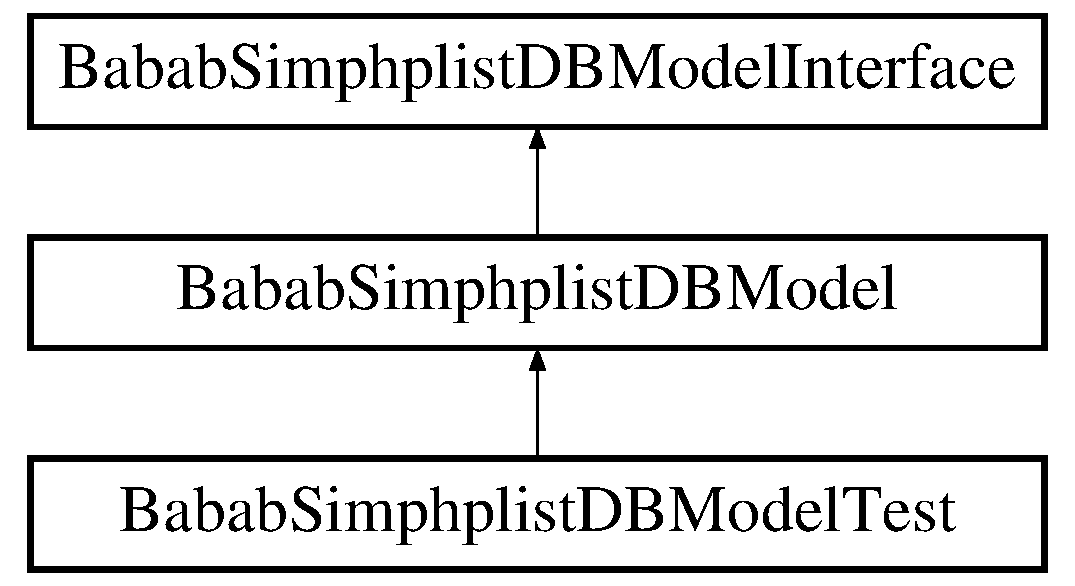
\includegraphics[height=3.000000cm]{classBabab_1_1Simphplist_1_1DB_1_1Model}
\end{center}
\end{figure}
\subsection*{Public Member Functions}
\begin{DoxyCompactItemize}
\item 
\hypertarget{classBabab_1_1Simphplist_1_1DB_1_1Model_a661b8c733241ca8031195fe5a71b3ec4}{{\bfseries \+\_\+\+\_\+construct} (\hyperlink{classBabab_1_1Simphplist_1_1DB_1_1MysqlHandler}{Mysql\+Handler} \$db)}\label{classBabab_1_1Simphplist_1_1DB_1_1Model_a661b8c733241ca8031195fe5a71b3ec4}

\item 
\hypertarget{classBabab_1_1Simphplist_1_1DB_1_1Model_a9d9f042b1ec3358a6b2c5f81ca335b87}{{\bfseries is\+Valid} ()}\label{classBabab_1_1Simphplist_1_1DB_1_1Model_a9d9f042b1ec3358a6b2c5f81ca335b87}

\item 
\hypertarget{classBabab_1_1Simphplist_1_1DB_1_1Model_a6940e9d2fcd0940e700bd96309718bc0}{{\bfseries get\+Validation\+Errors} ()}\label{classBabab_1_1Simphplist_1_1DB_1_1Model_a6940e9d2fcd0940e700bd96309718bc0}

\item 
\hypertarget{classBabab_1_1Simphplist_1_1DB_1_1Model_ab390eb521865138e82061a75ea75534e}{{\bfseries print\+Sql} ()}\label{classBabab_1_1Simphplist_1_1DB_1_1Model_ab390eb521865138e82061a75ea75534e}

\item 
\hypertarget{classBabab_1_1Simphplist_1_1DB_1_1Model_ab43d7cccf1a6bb05ef8c0e356fc73698}{{\bfseries print\+Info} ()}\label{classBabab_1_1Simphplist_1_1DB_1_1Model_ab43d7cccf1a6bb05ef8c0e356fc73698}

\end{DoxyCompactItemize}
\subsection*{Public Attributes}
\begin{DoxyCompactItemize}
\item 
\hypertarget{classBabab_1_1Simphplist_1_1DB_1_1Model_a0d4eb5374d3ecfe379cdf7a9c58af6ce}{{\bfseries \$\+\_\+table\+Name}}\label{classBabab_1_1Simphplist_1_1DB_1_1Model_a0d4eb5374d3ecfe379cdf7a9c58af6ce}

\end{DoxyCompactItemize}


\subsection{Detailed Description}
Object Mapper -- Abstract base class for writing Models that will be mapped to database tables. 

It acts like most O\+R\+M's but does not handle relations and has a unique D\+R\+Y approach to defining model properties and interacting with the exposed A\+P\+I. 

The documentation for this class was generated from the following file\+:\begin{DoxyCompactItemize}
\item 
/srv/http/simphplist/src/\+Babab/\+Simphplist/\+D\+B/Model.\+php\end{DoxyCompactItemize}

\hypertarget{interfaceBabab_1_1Simphplist_1_1DB_1_1ModelInterface}{\section{Babab\textbackslash{}Simphplist\textbackslash{}D\+B\textbackslash{}Model\+Interface Class Reference}
\label{interfaceBabab_1_1Simphplist_1_1DB_1_1ModelInterface}\index{Babab\textbackslash{}\+Simphplist\textbackslash{}\+D\+B\textbackslash{}\+Model\+Interface@{Babab\textbackslash{}\+Simphplist\textbackslash{}\+D\+B\textbackslash{}\+Model\+Interface}}
}


P\+H\+P Interface for abstract base class \hyperlink{classBabab_1_1Simphplist_1_1DB_1_1Model}{Model}.  


Inheritance diagram for Babab\textbackslash{}Simphplist\textbackslash{}D\+B\textbackslash{}Model\+Interface\+:\begin{figure}[H]
\begin{center}
\leavevmode
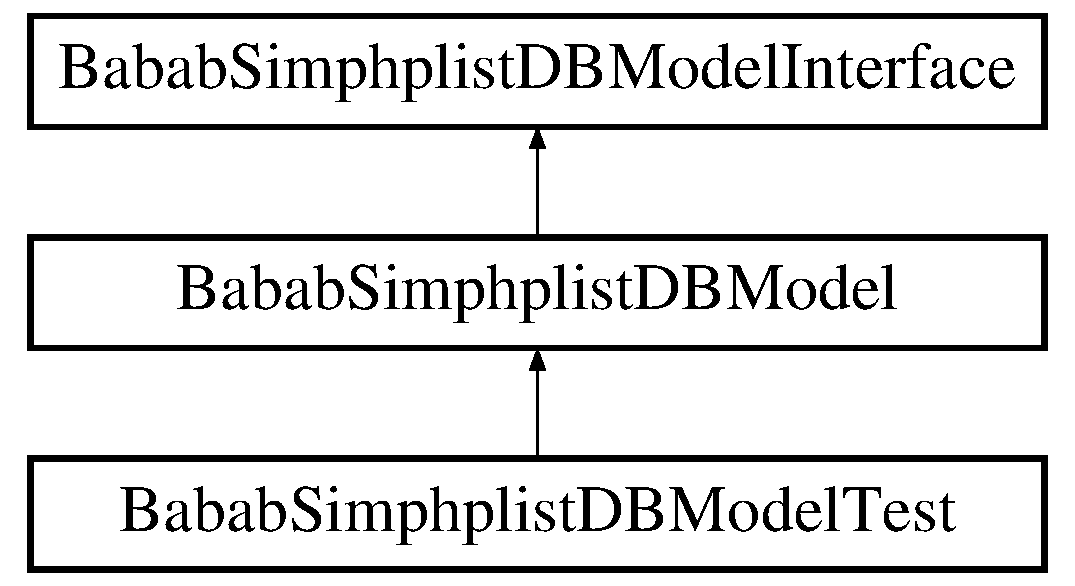
\includegraphics[height=3.000000cm]{interfaceBabab_1_1Simphplist_1_1DB_1_1ModelInterface}
\end{center}
\end{figure}
\subsection*{Public Member Functions}
\begin{DoxyCompactItemize}
\item 
\hypertarget{interfaceBabab_1_1Simphplist_1_1DB_1_1ModelInterface_a54775ae8d7e293b4ec842e6212db46e3}{{\bfseries \+\_\+\+\_\+construct} (\hyperlink{classBabab_1_1Simphplist_1_1DB_1_1MysqlHandler}{Mysql\+Handler} \$db)}\label{interfaceBabab_1_1Simphplist_1_1DB_1_1ModelInterface_a54775ae8d7e293b4ec842e6212db46e3}

\item 
\hypertarget{interfaceBabab_1_1Simphplist_1_1DB_1_1ModelInterface_a0d553ffa3355ceb92e013d686a9b17dc}{{\bfseries is\+Valid} ()}\label{interfaceBabab_1_1Simphplist_1_1DB_1_1ModelInterface_a0d553ffa3355ceb92e013d686a9b17dc}

\item 
\hypertarget{interfaceBabab_1_1Simphplist_1_1DB_1_1ModelInterface_aef40b6c9c160ee49de1eaa907fc8a8bb}{{\bfseries print\+Sql} ()}\label{interfaceBabab_1_1Simphplist_1_1DB_1_1ModelInterface_aef40b6c9c160ee49de1eaa907fc8a8bb}

\item 
\hypertarget{interfaceBabab_1_1Simphplist_1_1DB_1_1ModelInterface_a431764cc7cccba0688a7a969caa03dfb}{{\bfseries print\+Info} ()}\label{interfaceBabab_1_1Simphplist_1_1DB_1_1ModelInterface_a431764cc7cccba0688a7a969caa03dfb}

\end{DoxyCompactItemize}


\subsection{Detailed Description}
P\+H\+P Interface for abstract base class \hyperlink{classBabab_1_1Simphplist_1_1DB_1_1Model}{Model}. 

The documentation for this class was generated from the following file\+:\begin{DoxyCompactItemize}
\item 
/srv/http/simphplist/src/\+Babab/\+Simphplist/\+D\+B/Model.\+php\end{DoxyCompactItemize}

\hypertarget{classBabab_1_1Simphplist_1_1DB_1_1ModelTest}{\section{Babab\textbackslash{}Simphplist\textbackslash{}D\+B\textbackslash{}Model\+Test Class Reference}
\label{classBabab_1_1Simphplist_1_1DB_1_1ModelTest}\index{Babab\textbackslash{}\+Simphplist\textbackslash{}\+D\+B\textbackslash{}\+Model\+Test@{Babab\textbackslash{}\+Simphplist\textbackslash{}\+D\+B\textbackslash{}\+Model\+Test}}
}


Test model used as code example / for unit testing.  


Inheritance diagram for Babab\textbackslash{}Simphplist\textbackslash{}D\+B\textbackslash{}Model\+Test\+:\begin{figure}[H]
\begin{center}
\leavevmode
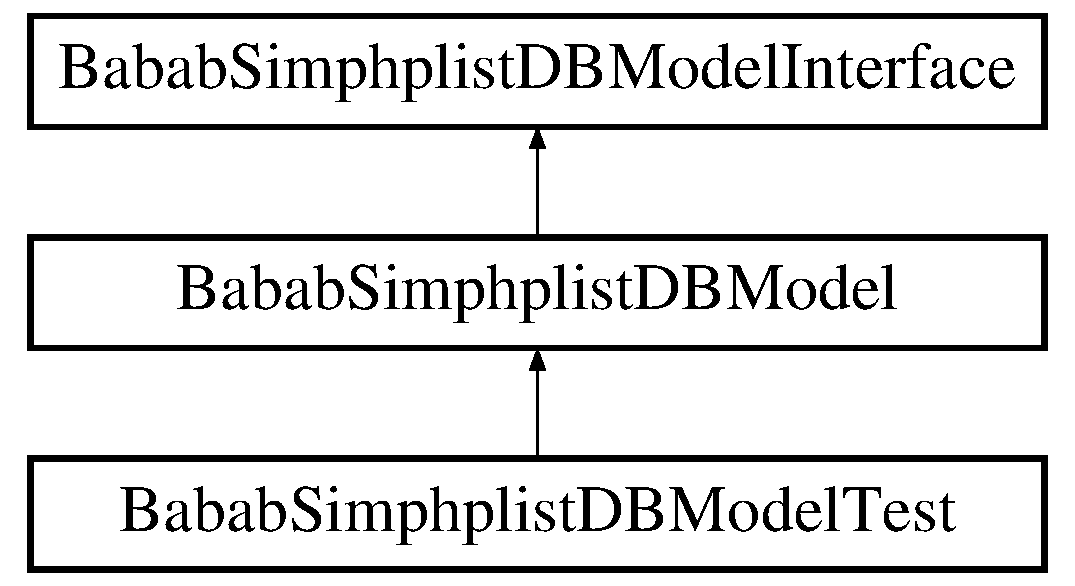
\includegraphics[height=3.000000cm]{classBabab_1_1Simphplist_1_1DB_1_1ModelTest}
\end{center}
\end{figure}
\subsection*{Public Attributes}
\begin{DoxyCompactItemize}
\item 
{\bfseries \$id}
\item 
{\bfseries \$title}
\item 
{\bfseries \$article\+Body}
\item 
{\bfseries \$newsletter}
\item 
{\bfseries \$sort\+Id}
\end{DoxyCompactItemize}
\subsection*{Additional Inherited Members}


\subsection{Detailed Description}
Test model used as code example / for unit testing. 

\subsection{Member Data Documentation}
\hypertarget{classBabab_1_1Simphplist_1_1DB_1_1ModelTest_af8a50d406da8bc9621d8419b9dca3b8b}{\index{Babab\+::\+Simphplist\+::\+D\+B\+::\+Model\+Test@{Babab\+::\+Simphplist\+::\+D\+B\+::\+Model\+Test}!\$article\+Body@{\$article\+Body}}
\index{\$article\+Body@{\$article\+Body}!Babab\+::\+Simphplist\+::\+D\+B\+::\+Model\+Test@{Babab\+::\+Simphplist\+::\+D\+B\+::\+Model\+Test}}
\subsubsection[{\$article\+Body}]{\setlength{\rightskip}{0pt plus 5cm}Babab\+::\+Simphplist\+::\+D\+B\textbackslash{}\+Model\+Test\+::\$article\+Body}}\label{classBabab_1_1Simphplist_1_1DB_1_1ModelTest_af8a50d406da8bc9621d8419b9dca3b8b}
{\bfseries Initial value\+:}
\begin{DoxyCode}
= array(
        \textcolor{stringliteral}{'type'} => \textcolor{stringliteral}{'text'},
    )
\end{DoxyCode}
\hypertarget{classBabab_1_1Simphplist_1_1DB_1_1ModelTest_a74473b58bab06575c6ed288d1058bcba}{\index{Babab\+::\+Simphplist\+::\+D\+B\+::\+Model\+Test@{Babab\+::\+Simphplist\+::\+D\+B\+::\+Model\+Test}!\$id@{\$id}}
\index{\$id@{\$id}!Babab\+::\+Simphplist\+::\+D\+B\+::\+Model\+Test@{Babab\+::\+Simphplist\+::\+D\+B\+::\+Model\+Test}}
\subsubsection[{\$id}]{\setlength{\rightskip}{0pt plus 5cm}Babab\+::\+Simphplist\+::\+D\+B\textbackslash{}\+Model\+Test\+::\$id}}\label{classBabab_1_1Simphplist_1_1DB_1_1ModelTest_a74473b58bab06575c6ed288d1058bcba}
{\bfseries Initial value\+:}
\begin{DoxyCode}
= array(
        \textcolor{stringliteral}{'type'} => \textcolor{stringliteral}{'int'},
        \textcolor{stringliteral}{'length'} => 11,
        \textcolor{stringliteral}{'null'} => False,
        \textcolor{stringliteral}{'primary\_key'} => True,
        \textcolor{stringliteral}{'auto\_increment'} => True,
    )
\end{DoxyCode}
\hypertarget{classBabab_1_1Simphplist_1_1DB_1_1ModelTest_afb73d61c30e855d47420a5ae76966c20}{\index{Babab\+::\+Simphplist\+::\+D\+B\+::\+Model\+Test@{Babab\+::\+Simphplist\+::\+D\+B\+::\+Model\+Test}!\$newsletter@{\$newsletter}}
\index{\$newsletter@{\$newsletter}!Babab\+::\+Simphplist\+::\+D\+B\+::\+Model\+Test@{Babab\+::\+Simphplist\+::\+D\+B\+::\+Model\+Test}}
\subsubsection[{\$newsletter}]{\setlength{\rightskip}{0pt plus 5cm}Babab\+::\+Simphplist\+::\+D\+B\textbackslash{}\+Model\+Test\+::\$newsletter}}\label{classBabab_1_1Simphplist_1_1DB_1_1ModelTest_afb73d61c30e855d47420a5ae76966c20}
{\bfseries Initial value\+:}
\begin{DoxyCode}
= array(
        \textcolor{stringliteral}{'type'} => \textcolor{stringliteral}{'boolean'},
        \textcolor{stringliteral}{'default'} => True,
    )
\end{DoxyCode}
\hypertarget{classBabab_1_1Simphplist_1_1DB_1_1ModelTest_afe0dd7be959f444f69bf7593c8c64fcd}{\index{Babab\+::\+Simphplist\+::\+D\+B\+::\+Model\+Test@{Babab\+::\+Simphplist\+::\+D\+B\+::\+Model\+Test}!\$sort\+Id@{\$sort\+Id}}
\index{\$sort\+Id@{\$sort\+Id}!Babab\+::\+Simphplist\+::\+D\+B\+::\+Model\+Test@{Babab\+::\+Simphplist\+::\+D\+B\+::\+Model\+Test}}
\subsubsection[{\$sort\+Id}]{\setlength{\rightskip}{0pt plus 5cm}Babab\+::\+Simphplist\+::\+D\+B\textbackslash{}\+Model\+Test\+::\$sort\+Id}}\label{classBabab_1_1Simphplist_1_1DB_1_1ModelTest_afe0dd7be959f444f69bf7593c8c64fcd}
{\bfseries Initial value\+:}
\begin{DoxyCode}
= array(
        \textcolor{stringliteral}{'type'} => \textcolor{stringliteral}{'int'},
        \textcolor{stringliteral}{'length'} => \textcolor{stringliteral}{'11'},
        \textcolor{stringliteral}{'default'} => -1,
    )
\end{DoxyCode}
\hypertarget{classBabab_1_1Simphplist_1_1DB_1_1ModelTest_a145f1e9466b264e70af26b16718ad6f1}{\index{Babab\+::\+Simphplist\+::\+D\+B\+::\+Model\+Test@{Babab\+::\+Simphplist\+::\+D\+B\+::\+Model\+Test}!\$title@{\$title}}
\index{\$title@{\$title}!Babab\+::\+Simphplist\+::\+D\+B\+::\+Model\+Test@{Babab\+::\+Simphplist\+::\+D\+B\+::\+Model\+Test}}
\subsubsection[{\$title}]{\setlength{\rightskip}{0pt plus 5cm}Babab\+::\+Simphplist\+::\+D\+B\textbackslash{}\+Model\+Test\+::\$title}}\label{classBabab_1_1Simphplist_1_1DB_1_1ModelTest_a145f1e9466b264e70af26b16718ad6f1}
{\bfseries Initial value\+:}
\begin{DoxyCode}
= array(
        
        
        \textcolor{stringliteral}{'unique\_key'} => True,
    )
\end{DoxyCode}


The documentation for this class was generated from the following file\+:\begin{DoxyCompactItemize}
\item 
/srv/http/simphplist/src/\+Babab/\+Simphplist/\+D\+B/Model\+Test.\+php\end{DoxyCompactItemize}

\hypertarget{classBabab_1_1Simphplist_1_1DB_1_1MysqlHandler}{\section{Babab\textbackslash{}Simphplist\textbackslash{}D\+B\textbackslash{}Mysql\+Handler Class Reference}
\label{classBabab_1_1Simphplist_1_1DB_1_1MysqlHandler}\index{Babab\textbackslash{}\+Simphplist\textbackslash{}\+D\+B\textbackslash{}\+Mysql\+Handler@{Babab\textbackslash{}\+Simphplist\textbackslash{}\+D\+B\textbackslash{}\+Mysql\+Handler}}
}


My\+S\+Q\+L Handler with table prefix support.  


\subsection*{Public Member Functions}
\begin{DoxyCompactItemize}
\item 
\hyperlink{classBabab_1_1Simphplist_1_1DB_1_1MysqlHandler_ace2ba4301dbdbe8b3c9cfd3297816394}{\+\_\+\+\_\+construct} (\$mysqli\+\_\+or\+\_\+settings=Null)
\item 
\hyperlink{classBabab_1_1Simphplist_1_1DB_1_1MysqlHandler_af75512d0141b5f9256677ad5737b6505}{query} (\$query)
\item 
\hyperlink{classBabab_1_1Simphplist_1_1DB_1_1MysqlHandler_abfca7a1443ab42be5b4104a81f12530f}{q} (\$\hyperlink{classBabab_1_1Simphplist_1_1DB_1_1MysqlHandler_af75512d0141b5f9256677ad5737b6505}{query})
\item 
\hyperlink{classBabab_1_1Simphplist_1_1DB_1_1MysqlHandler_a4bc07f585cd897c60d4cb84040a3582c}{qfetch} (\$\hyperlink{classBabab_1_1Simphplist_1_1DB_1_1MysqlHandler_af75512d0141b5f9256677ad5737b6505}{query}, \$order=False, \$reverse\+\_\+order=False)
\item 
\hypertarget{classBabab_1_1Simphplist_1_1DB_1_1MysqlHandler_aa45de5f4f088dbb0c2d196ebb16a3a03}{{\bfseries set\+Prefix} (\$prefix)}\label{classBabab_1_1Simphplist_1_1DB_1_1MysqlHandler_aa45de5f4f088dbb0c2d196ebb16a3a03}

\item 
\hypertarget{classBabab_1_1Simphplist_1_1DB_1_1MysqlHandler_a81e4b91e84ce126150633a0a2e6e43f6}{{\bfseries get\+Prefix} ()}\label{classBabab_1_1Simphplist_1_1DB_1_1MysqlHandler_a81e4b91e84ce126150633a0a2e6e43f6}

\item 
\hypertarget{classBabab_1_1Simphplist_1_1DB_1_1MysqlHandler_a0cbfc05764cd89a6652c5c1e7fd872b9}{{\bfseries set\+Prefix\+Replace\+String} (\$prefix\+Replace\+String)}\label{classBabab_1_1Simphplist_1_1DB_1_1MysqlHandler_a0cbfc05764cd89a6652c5c1e7fd872b9}

\item 
\hypertarget{classBabab_1_1Simphplist_1_1DB_1_1MysqlHandler_a5e3abb0cd1ec78becae635de0eb349a1}{{\bfseries close} ()}\label{classBabab_1_1Simphplist_1_1DB_1_1MysqlHandler_a5e3abb0cd1ec78becae635de0eb349a1}

\item 
\hypertarget{classBabab_1_1Simphplist_1_1DB_1_1MysqlHandler_ab363ecda5a04efe240e32a4e4e3ddcf7}{{\bfseries info} ()}\label{classBabab_1_1Simphplist_1_1DB_1_1MysqlHandler_ab363ecda5a04efe240e32a4e4e3ddcf7}

\end{DoxyCompactItemize}


\subsection{Detailed Description}
My\+S\+Q\+L Handler with table prefix support. 

\subsection{Constructor \& Destructor Documentation}
\hypertarget{classBabab_1_1Simphplist_1_1DB_1_1MysqlHandler_ace2ba4301dbdbe8b3c9cfd3297816394}{\index{Babab\+::\+Simphplist\+::\+D\+B\+::\+Mysql\+Handler@{Babab\+::\+Simphplist\+::\+D\+B\+::\+Mysql\+Handler}!\+\_\+\+\_\+construct@{\+\_\+\+\_\+construct}}
\index{\+\_\+\+\_\+construct@{\+\_\+\+\_\+construct}!Babab\+::\+Simphplist\+::\+D\+B\+::\+Mysql\+Handler@{Babab\+::\+Simphplist\+::\+D\+B\+::\+Mysql\+Handler}}
\subsubsection[{\+\_\+\+\_\+construct}]{\setlength{\rightskip}{0pt plus 5cm}Babab\textbackslash{}\+Simphplist\textbackslash{}\+D\+B\textbackslash{}\+Mysql\+Handler\+::\+\_\+\+\_\+construct (
\begin{DoxyParamCaption}
\item[{}]{\$mysqli\+\_\+or\+\_\+settings = {\ttfamily Null}}
\end{DoxyParamCaption}
)}}\label{classBabab_1_1Simphplist_1_1DB_1_1MysqlHandler_ace2ba4301dbdbe8b3c9cfd3297816394}
Constructor for \hyperlink{classBabab_1_1Simphplist_1_1DB_1_1MysqlHandler}{Mysql\+Handler}


\begin{DoxyParams}[1]{Parameters}
\textbackslash{}mysqli  |  array & {\em \$mysqli\+\_\+or\+\_\+settings} & mysqli instance or settings array \\
\hline
\end{DoxyParams}


\subsection{Member Function Documentation}
\hypertarget{classBabab_1_1Simphplist_1_1DB_1_1MysqlHandler_abfca7a1443ab42be5b4104a81f12530f}{\index{Babab\+::\+Simphplist\+::\+D\+B\+::\+Mysql\+Handler@{Babab\+::\+Simphplist\+::\+D\+B\+::\+Mysql\+Handler}!q@{q}}
\index{q@{q}!Babab\+::\+Simphplist\+::\+D\+B\+::\+Mysql\+Handler@{Babab\+::\+Simphplist\+::\+D\+B\+::\+Mysql\+Handler}}
\subsubsection[{q}]{\setlength{\rightskip}{0pt plus 5cm}Babab\textbackslash{}\+Simphplist\textbackslash{}\+D\+B\textbackslash{}\+Mysql\+Handler\+::q (
\begin{DoxyParamCaption}
\item[{}]{\$query}
\end{DoxyParamCaption}
)}}\label{classBabab_1_1Simphplist_1_1DB_1_1MysqlHandler_abfca7a1443ab42be5b4104a81f12530f}
Execute query after substituting prefix; Alias for this\+::query()


\begin{DoxyParams}[1]{Parameters}
string & {\em \$query} & Query string (optionally prefixed with \$this-\/$>$\+\_\+prefix\+Replace\+String) \\
\hline
\end{DoxyParams}
\begin{DoxyReturn}{Returns}
\+::query Query result 
\end{DoxyReturn}
\hypertarget{classBabab_1_1Simphplist_1_1DB_1_1MysqlHandler_a4bc07f585cd897c60d4cb84040a3582c}{\index{Babab\+::\+Simphplist\+::\+D\+B\+::\+Mysql\+Handler@{Babab\+::\+Simphplist\+::\+D\+B\+::\+Mysql\+Handler}!qfetch@{qfetch}}
\index{qfetch@{qfetch}!Babab\+::\+Simphplist\+::\+D\+B\+::\+Mysql\+Handler@{Babab\+::\+Simphplist\+::\+D\+B\+::\+Mysql\+Handler}}
\subsubsection[{qfetch}]{\setlength{\rightskip}{0pt plus 5cm}Babab\textbackslash{}\+Simphplist\textbackslash{}\+D\+B\textbackslash{}\+Mysql\+Handler\+::qfetch (
\begin{DoxyParamCaption}
\item[{}]{\$query, }
\item[{}]{\$order = {\ttfamily False}, }
\item[{}]{\$reverse\+\_\+order = {\ttfamily False}}
\end{DoxyParamCaption}
)}}\label{classBabab_1_1Simphplist_1_1DB_1_1MysqlHandler_a4bc07f585cd897c60d4cb84040a3582c}
Execute a query and return results as a (multi-\/dimensonal) associative array


\begin{DoxyParams}[1]{Parameters}
string & {\em \$query} & Query string (optionally prefixed with \$this-\/$>$\+\_\+prefix\+Replace\+String) \\
\hline
bool & {\em \$order} & Sort results \\
\hline
bool & {\em \$reverse\+\_\+order} & Reverse sort results\\
\hline
\end{DoxyParams}
\begin{DoxyReturn}{Returns}
array 
\end{DoxyReturn}
\hypertarget{classBabab_1_1Simphplist_1_1DB_1_1MysqlHandler_af75512d0141b5f9256677ad5737b6505}{\index{Babab\+::\+Simphplist\+::\+D\+B\+::\+Mysql\+Handler@{Babab\+::\+Simphplist\+::\+D\+B\+::\+Mysql\+Handler}!query@{query}}
\index{query@{query}!Babab\+::\+Simphplist\+::\+D\+B\+::\+Mysql\+Handler@{Babab\+::\+Simphplist\+::\+D\+B\+::\+Mysql\+Handler}}
\subsubsection[{query}]{\setlength{\rightskip}{0pt plus 5cm}Babab\textbackslash{}\+Simphplist\textbackslash{}\+D\+B\textbackslash{}\+Mysql\+Handler\+::query (
\begin{DoxyParamCaption}
\item[{}]{\$query}
\end{DoxyParamCaption}
)}}\label{classBabab_1_1Simphplist_1_1DB_1_1MysqlHandler_af75512d0141b5f9256677ad5737b6505}
Execute query after substituting prefix


\begin{DoxyParams}[1]{Parameters}
string & {\em \$query} & Query string (optionally prefixed with \$this-\/$>$\+\_\+prefix\+Replace\+String) \\
\hline
\end{DoxyParams}
\begin{DoxyReturn}{Returns}
\+::query Query result 
\end{DoxyReturn}


The documentation for this class was generated from the following file\+:\begin{DoxyCompactItemize}
\item 
/srv/http/simphplist/src/\+Babab/\+Simphplist/\+D\+B/Mysql\+Handler.\+php\end{DoxyCompactItemize}

\hypertarget{classBabab_1_1Simphplist_1_1Request}{\section{Babab\textbackslash{}Simphplist\textbackslash{}Request Class Reference}
\label{classBabab_1_1Simphplist_1_1Request}\index{Babab\textbackslash{}\+Simphplist\textbackslash{}\+Request@{Babab\textbackslash{}\+Simphplist\textbackslash{}\+Request}}
}


Static methods for secure user input handling via R\+E\+Q\+U\+E\+S\+T superglobal(s)\+: (G\+E\+T, P\+O\+S\+T, C\+O\+O\+K\+I\+E)  


\subsection*{Static Public Member Functions}
\begin{DoxyCompactItemize}
\item 
\hypertarget{classBabab_1_1Simphplist_1_1Request_a3516c95fe4531c57e099e447749a5202}{static {\bfseries get} (\$var, \$default\+Value='')}\label{classBabab_1_1Simphplist_1_1Request_a3516c95fe4531c57e099e447749a5202}

\item 
\hypertarget{classBabab_1_1Simphplist_1_1Request_a0d5005e76b41f9515493e77845555078}{static {\bfseries post} (\$var, \$default\+Value='')}\label{classBabab_1_1Simphplist_1_1Request_a0d5005e76b41f9515493e77845555078}

\end{DoxyCompactItemize}


\subsection{Detailed Description}
Static methods for secure user input handling via R\+E\+Q\+U\+E\+S\+T superglobal(s)\+: (G\+E\+T, P\+O\+S\+T, C\+O\+O\+K\+I\+E) 

The documentation for this class was generated from the following file\+:\begin{DoxyCompactItemize}
\item 
/srv/http/simphplist/src/\+Babab/\+Simphplist/Request.\+php\end{DoxyCompactItemize}

\hypertarget{classBabab_1_1Simphplist_1_1Route}{\section{Babab\textbackslash{}Simphplist\textbackslash{}Route Class Reference}
\label{classBabab_1_1Simphplist_1_1Route}\index{Babab\textbackslash{}\+Simphplist\textbackslash{}\+Route@{Babab\textbackslash{}\+Simphplist\textbackslash{}\+Route}}
}


Minimalistic, flexible and extensible routing.  


\subsection*{Public Member Functions}
\begin{DoxyCompactItemize}
\item 
\hyperlink{classBabab_1_1Simphplist_1_1Route_a998abb044d2a0d1ef2b2c1bc727c475e}{other} (\$func)
\item 
\hyperlink{classBabab_1_1Simphplist_1_1Route_ae51d0a0c3732e3778fa02ef0c3ca2d54}{when} ()
\item 
\hypertarget{classBabab_1_1Simphplist_1_1Route_a04976cbc3bec89b44e23616abf61753e}{{\bfseries set\+Prefix} (\$prefix)}\label{classBabab_1_1Simphplist_1_1Route_a04976cbc3bec89b44e23616abf61753e}

\item 
\hyperlink{classBabab_1_1Simphplist_1_1Route_a081a289530000948636ab410e682f335}{parse\+U\+R\+I} (\$reference\+Path)
\end{DoxyCompactItemize}
\subsection*{Static Public Member Functions}
\begin{DoxyCompactItemize}
\item 
\hypertarget{classBabab_1_1Simphplist_1_1Route_a295f532ff277469fb2560be8333e9d2b}{static {\bfseries redirect} (\$uri, \$http\+Prefixer=false)}\label{classBabab_1_1Simphplist_1_1Route_a295f532ff277469fb2560be8333e9d2b}

\end{DoxyCompactItemize}


\subsection{Detailed Description}
Minimalistic, flexible and extensible routing. 

\subsection{Member Function Documentation}
\hypertarget{classBabab_1_1Simphplist_1_1Route_a998abb044d2a0d1ef2b2c1bc727c475e}{\index{Babab\+::\+Simphplist\+::\+Route@{Babab\+::\+Simphplist\+::\+Route}!other@{other}}
\index{other@{other}!Babab\+::\+Simphplist\+::\+Route@{Babab\+::\+Simphplist\+::\+Route}}
\subsubsection[{other}]{\setlength{\rightskip}{0pt plus 5cm}Babab\textbackslash{}\+Simphplist\textbackslash{}\+Route\+::other (
\begin{DoxyParamCaption}
\item[{}]{\$func}
\end{DoxyParamCaption}
)}}\label{classBabab_1_1Simphplist_1_1Route_a998abb044d2a0d1ef2b2c1bc727c475e}
Run a default closure when no other previous {\ttfamily \hyperlink{classBabab_1_1Simphplist_1_1Route_ae51d0a0c3732e3778fa02ef0c3ca2d54}{when()}} calls have matched. The closure cannot accept arguments.


\begin{DoxyParams}[1]{Parameters}
callable & {\em \$func} & A closure or variable function to run \\
\hline
\end{DoxyParams}

\begin{DoxyRetVals}{Return values}
{\em bool} & $\vert$ array Match success or matched identifier pair \\
\hline
\end{DoxyRetVals}
\hypertarget{classBabab_1_1Simphplist_1_1Route_a081a289530000948636ab410e682f335}{\index{Babab\+::\+Simphplist\+::\+Route@{Babab\+::\+Simphplist\+::\+Route}!parse\+U\+R\+I@{parse\+U\+R\+I}}
\index{parse\+U\+R\+I@{parse\+U\+R\+I}!Babab\+::\+Simphplist\+::\+Route@{Babab\+::\+Simphplist\+::\+Route}}
\subsubsection[{parse\+U\+R\+I}]{\setlength{\rightskip}{0pt plus 5cm}Babab\textbackslash{}\+Simphplist\textbackslash{}\+Route\+::parse\+U\+R\+I (
\begin{DoxyParamCaption}
\item[{}]{\$reference\+Path}
\end{DoxyParamCaption}
)}}\label{classBabab_1_1Simphplist_1_1Route_a081a289530000948636ab410e682f335}
Match R\+E\+Q\+U\+E\+S\+T\+\_\+\+U\+R\+I with \$reference path

The R\+E\+Q\+U\+E\+S\+T\+\_\+\+U\+R\+I is optionally stripped with prefix before matching (useful for developing without rewriting rules, with P\+H\+P's built in webserver for example)

Returns an object with matched identifier pairs when applicable; Returns true then a match is found without identifiers; Returns false when no match is found


\begin{DoxyParams}[1]{Parameters}
string & {\em \$reference\+Path} & The U\+R\+I format to match for \\
\hline
\end{DoxyParams}

\begin{DoxyRetVals}{Return values}
{\em bool} & $\vert$ array Match success or matched identifier pair \\
\hline
\end{DoxyRetVals}
\hypertarget{classBabab_1_1Simphplist_1_1Route_ae51d0a0c3732e3778fa02ef0c3ca2d54}{\index{Babab\+::\+Simphplist\+::\+Route@{Babab\+::\+Simphplist\+::\+Route}!when@{when}}
\index{when@{when}!Babab\+::\+Simphplist\+::\+Route@{Babab\+::\+Simphplist\+::\+Route}}
\subsubsection[{when}]{\setlength{\rightskip}{0pt plus 5cm}Babab\textbackslash{}\+Simphplist\textbackslash{}\+Route\+::when (
\begin{DoxyParamCaption}
{}
\end{DoxyParamCaption}
)}}\label{classBabab_1_1Simphplist_1_1Route_ae51d0a0c3732e3778fa02ef0c3ca2d54}
Run a closure when the visited U\+R\+L matches the defined U\+R\+I format

An \$uri can have identifiers, which are marked with {\ttfamily \{\}}. In the following example there is an 'id' identifier for a blog article\+: \begin{DoxyVerb}(new \Babab\Simphplist\Routing\Route)

->when('/blog/articles/{id}/, function($someArray) {
     echo 'This is article: ' . $someArray['id'];
})

->when('/blog/articles/, function($void) {
     echo 'This is the article list';
})

->other(function() {
    \Babab\Simphplist\Route::redirect('/blog/articles/');
});
\end{DoxyVerb}


When the url is matched, any values that are matched with identifiers are added to an object (with the identifiers as property names), which is in turn passed to the closure.

The closure should therefore always accept an (object as) argument.


\begin{DoxyParams}[1]{Parameters}
string & {\em \$uri} & The U\+R\+I format to match for \\
\hline
 & {\em ...} & optional arguments to pass to closure (N/\+A yet) \\
\hline
callable & {\em \$func} & A closure or variable function to run \\
\hline
\end{DoxyParams}

\begin{DoxyRetVals}{Return values}
{\em bool} & $\vert$ array Match success or matched identifier pair \\
\hline
\end{DoxyRetVals}


The documentation for this class was generated from the following file\+:\begin{DoxyCompactItemize}
\item 
/srv/http/simphplist/src/\+Babab/\+Simphplist/Route.\+php\end{DoxyCompactItemize}

\hypertarget{classBabab_1_1Simphplist_1_1String}{\section{Babab\textbackslash{}Simphplist\textbackslash{}String Class Reference}
\label{classBabab_1_1Simphplist_1_1String}\index{Babab\textbackslash{}\+Simphplist\textbackslash{}\+String@{Babab\textbackslash{}\+Simphplist\textbackslash{}\+String}}
}


Static methods for common string manipulation / parsing tasks.  


\subsection*{Static Public Member Functions}
\begin{DoxyCompactItemize}
\item 
static \hyperlink{classBabab_1_1Simphplist_1_1String_a142a5a5e92a03445871984f226917b8d}{truncate} (\$string, \$n\+Chars, \$suffix= '...')
\item 
\hypertarget{classBabab_1_1Simphplist_1_1String_a3c68e6bf2659b0d2ed213a8bbb8a964c}{static {\bfseries filter} (\$var, \$default\+Value='')}\label{classBabab_1_1Simphplist_1_1String_a3c68e6bf2659b0d2ed213a8bbb8a964c}

\item 
\hypertarget{classBabab_1_1Simphplist_1_1String_ae83af1a02810785685783d31cef89d8b}{static {\bfseries replace} (\$string, \$replace\+Array)}\label{classBabab_1_1Simphplist_1_1String_ae83af1a02810785685783d31cef89d8b}

\item 
\hypertarget{classBabab_1_1Simphplist_1_1String_aba448d2953a2460635a4f760c759fc0c}{static {\bfseries word\+Type} (\$word)}\label{classBabab_1_1Simphplist_1_1String_aba448d2953a2460635a4f760c759fc0c}

\item 
\hypertarget{classBabab_1_1Simphplist_1_1String_ada07abcb49a98db46fd776c6da8c473c}{static {\bfseries count} (\$text)}\label{classBabab_1_1Simphplist_1_1String_ada07abcb49a98db46fd776c6da8c473c}

\item 
\hypertarget{classBabab_1_1Simphplist_1_1String_a108a4baabcab44ce8dd27c573d052da0}{static {\bfseries cast} (\$string, \$cast\+To\+Type)}\label{classBabab_1_1Simphplist_1_1String_a108a4baabcab44ce8dd27c573d052da0}

\end{DoxyCompactItemize}
\subsection*{Public Attributes}
\begin{DoxyCompactItemize}
\item 
\hypertarget{classBabab_1_1Simphplist_1_1String_ac9a5b0f0ab6669f348d8fd4b7872d886}{const {\bfseries W\+O\+R\+D\+\_\+\+L\+O\+W\+E\+R\+C\+A\+S\+E} = 1}\label{classBabab_1_1Simphplist_1_1String_ac9a5b0f0ab6669f348d8fd4b7872d886}

\item 
\hypertarget{classBabab_1_1Simphplist_1_1String_a50cb0d79ad7c99ee26a5671a8c8d5155}{const {\bfseries W\+O\+R\+D\+\_\+\+C\+A\+P\+I\+T\+A\+L\+I\+Z\+E\+D} = 2}\label{classBabab_1_1Simphplist_1_1String_a50cb0d79ad7c99ee26a5671a8c8d5155}

\item 
\hypertarget{classBabab_1_1Simphplist_1_1String_a4ddd0903abb5cb79188a99c22029ff63}{const {\bfseries W\+O\+R\+D\+\_\+\+C\+A\+M\+E\+L\+C\+A\+S\+E} = 3}\label{classBabab_1_1Simphplist_1_1String_a4ddd0903abb5cb79188a99c22029ff63}

\item 
\hypertarget{classBabab_1_1Simphplist_1_1String_adba85d1760b3aea3506448855ec4e923}{const {\bfseries W\+O\+R\+D\+\_\+\+M\+I\+X\+E\+D\+C\+A\+S\+E} = 4}\label{classBabab_1_1Simphplist_1_1String_adba85d1760b3aea3506448855ec4e923}

\item 
\hypertarget{classBabab_1_1Simphplist_1_1String_a44f3604e9470b92f5f7f1128bba98f35}{const {\bfseries W\+O\+R\+D\+\_\+\+U\+P\+P\+E\+R\+C\+A\+S\+E} = 5}\label{classBabab_1_1Simphplist_1_1String_a44f3604e9470b92f5f7f1128bba98f35}

\end{DoxyCompactItemize}


\subsection{Detailed Description}
Static methods for common string manipulation / parsing tasks. 

\subsection{Member Function Documentation}
\hypertarget{classBabab_1_1Simphplist_1_1String_a142a5a5e92a03445871984f226917b8d}{\index{Babab\+::\+Simphplist\+::\+String@{Babab\+::\+Simphplist\+::\+String}!truncate@{truncate}}
\index{truncate@{truncate}!Babab\+::\+Simphplist\+::\+String@{Babab\+::\+Simphplist\+::\+String}}
\subsubsection[{truncate}]{\setlength{\rightskip}{0pt plus 5cm}static Babab\textbackslash{}\+Simphplist\textbackslash{}\+String\+::truncate (
\begin{DoxyParamCaption}
\item[{}]{\$string, }
\item[{}]{\$n\+Chars, }
\item[{}]{\$suffix = {\ttfamily '...'}}
\end{DoxyParamCaption}
)\hspace{0.3cm}{\ttfamily [static]}}}\label{classBabab_1_1Simphplist_1_1String_a142a5a5e92a03445871984f226917b8d}
Truncate a string if it exceeds a certain length

The string length of \$suffix is taken into account for the maximum number of chars \$n\+Chars this method will return.


\begin{DoxyParams}[1]{Parameters}
string & {\em \$string} & The string that is subject to truncation \\
\hline
int & {\em \$n\+Chars} & The maximum number of chars to return \\
\hline
string & {\em \$suffix} & A suffix string to indicate the truncation \\
\hline
\end{DoxyParams}

\begin{DoxyRetVals}{Return values}
{\em string} & A truncated version of \$string \\
\hline
\end{DoxyRetVals}


The documentation for this class was generated from the following file\+:\begin{DoxyCompactItemize}
\item 
/srv/http/simphplist/src/\+Babab/\+Simphplist/String.\+php\end{DoxyCompactItemize}

\hypertarget{classBabab_1_1SimphplistTests_1_1StringTest}{\section{Babab\textbackslash{}Simphplist\+Tests\textbackslash{}String\+Test Class Reference}
\label{classBabab_1_1SimphplistTests_1_1StringTest}\index{Babab\textbackslash{}\+Simphplist\+Tests\textbackslash{}\+String\+Test@{Babab\textbackslash{}\+Simphplist\+Tests\textbackslash{}\+String\+Test}}
}
Inheritance diagram for Babab\textbackslash{}Simphplist\+Tests\textbackslash{}String\+Test\+:\begin{figure}[H]
\begin{center}
\leavevmode
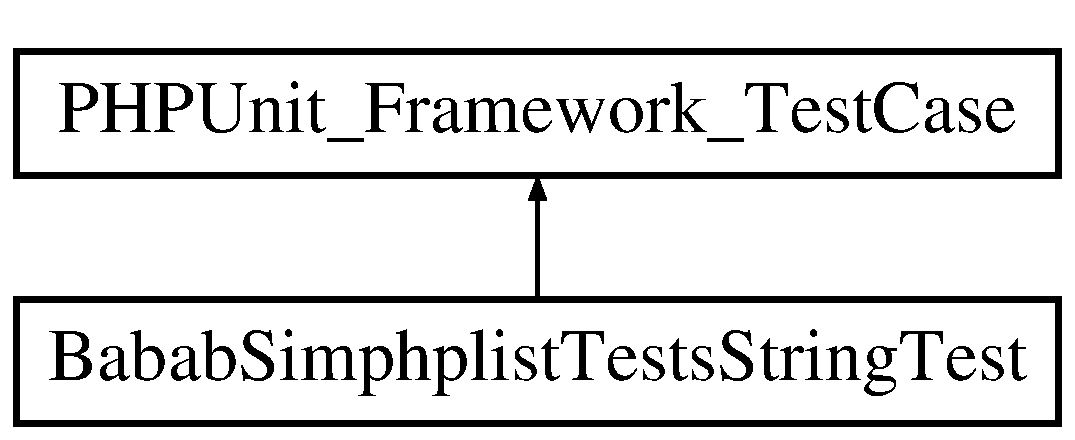
\includegraphics[height=2.000000cm]{classBabab_1_1SimphplistTests_1_1StringTest}
\end{center}
\end{figure}
\subsection*{Public Member Functions}
\begin{DoxyCompactItemize}
\item 
\hypertarget{classBabab_1_1SimphplistTests_1_1StringTest_a76d9ae67ee8ef0781a3f59ecc4496449}{{\bfseries test\+Filter} ()}\label{classBabab_1_1SimphplistTests_1_1StringTest_a76d9ae67ee8ef0781a3f59ecc4496449}

\end{DoxyCompactItemize}


The documentation for this class was generated from the following file\+:\begin{DoxyCompactItemize}
\item 
/srv/http/simphplist/tests/String\+Test.\+php\end{DoxyCompactItemize}

\hypertarget{classBabab_1_1Simphplist_1_1Validate}{\section{Babab\textbackslash{}Simphplist\textbackslash{}Validate Class Reference}
\label{classBabab_1_1Simphplist_1_1Validate}\index{Babab\textbackslash{}\+Simphplist\textbackslash{}\+Validate@{Babab\textbackslash{}\+Simphplist\textbackslash{}\+Validate}}
}


Clean static A\+P\+I for type checking and validation.  


\subsection*{Static Public Member Functions}
\begin{DoxyCompactItemize}
\item 
static \hyperlink{classBabab_1_1Simphplist_1_1Validate_a51cdfbb89af6ba182a21fb537b1e2aa5}{is\+Bool} (\$var, \$strict=true)
\item 
static \hyperlink{classBabab_1_1Simphplist_1_1Validate_a1b82b4c46c0409d8cfb2c57f11aac5e3}{is\+Time\+String} (\$var)
\end{DoxyCompactItemize}


\subsection{Detailed Description}
Clean static A\+P\+I for type checking and validation. 

\subsection{Member Function Documentation}
\hypertarget{classBabab_1_1Simphplist_1_1Validate_a51cdfbb89af6ba182a21fb537b1e2aa5}{\index{Babab\+::\+Simphplist\+::\+Validate@{Babab\+::\+Simphplist\+::\+Validate}!is\+Bool@{is\+Bool}}
\index{is\+Bool@{is\+Bool}!Babab\+::\+Simphplist\+::\+Validate@{Babab\+::\+Simphplist\+::\+Validate}}
\subsubsection[{is\+Bool}]{\setlength{\rightskip}{0pt plus 5cm}static Babab\textbackslash{}\+Simphplist\textbackslash{}\+Validate\+::is\+Bool (
\begin{DoxyParamCaption}
\item[{}]{\$var, }
\item[{}]{\$strict = {\ttfamily true}}
\end{DoxyParamCaption}
)\hspace{0.3cm}{\ttfamily [static]}}}\label{classBabab_1_1Simphplist_1_1Validate_a51cdfbb89af6ba182a21fb537b1e2aa5}
Checks if variable is a true boolean

This is an alias for P\+H\+P's {\ttfamily is\+\_\+bool} function adapted with a non strict test to allow case-\/insensitive strings of \char`\"{}true\char`\"{} and \char`\"{}false\char`\"{} to evaluate as true.


\begin{DoxyParams}[1]{Parameters}
mixed & {\em \$var} & The variable to test \\
\hline
bool & {\em \$strict} & The variable to test \\
\hline
\end{DoxyParams}
\begin{DoxyReturn}{Returns}
bool 
\end{DoxyReturn}
\hypertarget{classBabab_1_1Simphplist_1_1Validate_a1b82b4c46c0409d8cfb2c57f11aac5e3}{\index{Babab\+::\+Simphplist\+::\+Validate@{Babab\+::\+Simphplist\+::\+Validate}!is\+Time\+String@{is\+Time\+String}}
\index{is\+Time\+String@{is\+Time\+String}!Babab\+::\+Simphplist\+::\+Validate@{Babab\+::\+Simphplist\+::\+Validate}}
\subsubsection[{is\+Time\+String}]{\setlength{\rightskip}{0pt plus 5cm}static Babab\textbackslash{}\+Simphplist\textbackslash{}\+Validate\+::is\+Time\+String (
\begin{DoxyParamCaption}
\item[{}]{\$var}
\end{DoxyParamCaption}
)\hspace{0.3cm}{\ttfamily [static]}}}\label{classBabab_1_1Simphplist_1_1Validate_a1b82b4c46c0409d8cfb2c57f11aac5e3}
Checks if variable is a valid time string

Valid strings are\+: \char`\"{}18\+:34\char`\"{}, \char`\"{}09\+:00 am\char`\"{}, \char`\"{}8\+:34 P\+M\char`\"{}. Invalid strings are\+: \char`\"{}18\+:63\char`\"{}, \char`\"{}09\+:00 a\+M\char`\"{}, \char`\"{}20\+:34 P\+M\char`\"{}.


\begin{DoxyParams}[1]{Parameters}
mixed & {\em \$var} & The variable to test \\
\hline
\end{DoxyParams}
\begin{DoxyReturn}{Returns}
bool 
\end{DoxyReturn}


The documentation for this class was generated from the following file\+:\begin{DoxyCompactItemize}
\item 
/srv/http/simphplist/src/\+Babab/\+Simphplist/Validate.\+php\end{DoxyCompactItemize}

%--- End generated contents ---

% Index
\newpage
\phantomsection
\addcontentsline{toc}{chapter}{Index}
\printindex

\end{document}
